\documentclass{article}
\usepackage{graphicx} % Required for inserting images
\usepackage{fancyhdr}
\usepackage{minted}
\usepackage{amsmath}
\usepackage{hyperref}
\usepackage{listings}

\hypersetup{
    colorlinks=true,   % Farben statt Umrandung für Links
    linkcolor=black,    % Farbe für interne Links
    citecolor=blue,    % Farbe für Zitate
    filecolor=blue,    % Farbe für Dateien
    urlcolor=blue      % Farbe für URLs
}

\usepackage{array}
\pagestyle{fancy}
\title{Topic 1: Exon Skipping}
\author{1 \&  2 }
\date{October 2024}


\begin{document}

    \maketitle
    \tableofcontents
    \pagebreak


    \section{Introduction}
% Problembeschreibung/definition
    Alternative splicing is a process during gene expression that allows a single gene to produce different splice variants. For example, some gene exons may be included within or excluded from the final RNA product of the gene. This form of splicing is referred to as exon skipping. Detecting exon-skipping events is crucial for understanding the complexity of gene regulation and the functional diversity of proteins.

    \begin{figure}
        \centering
        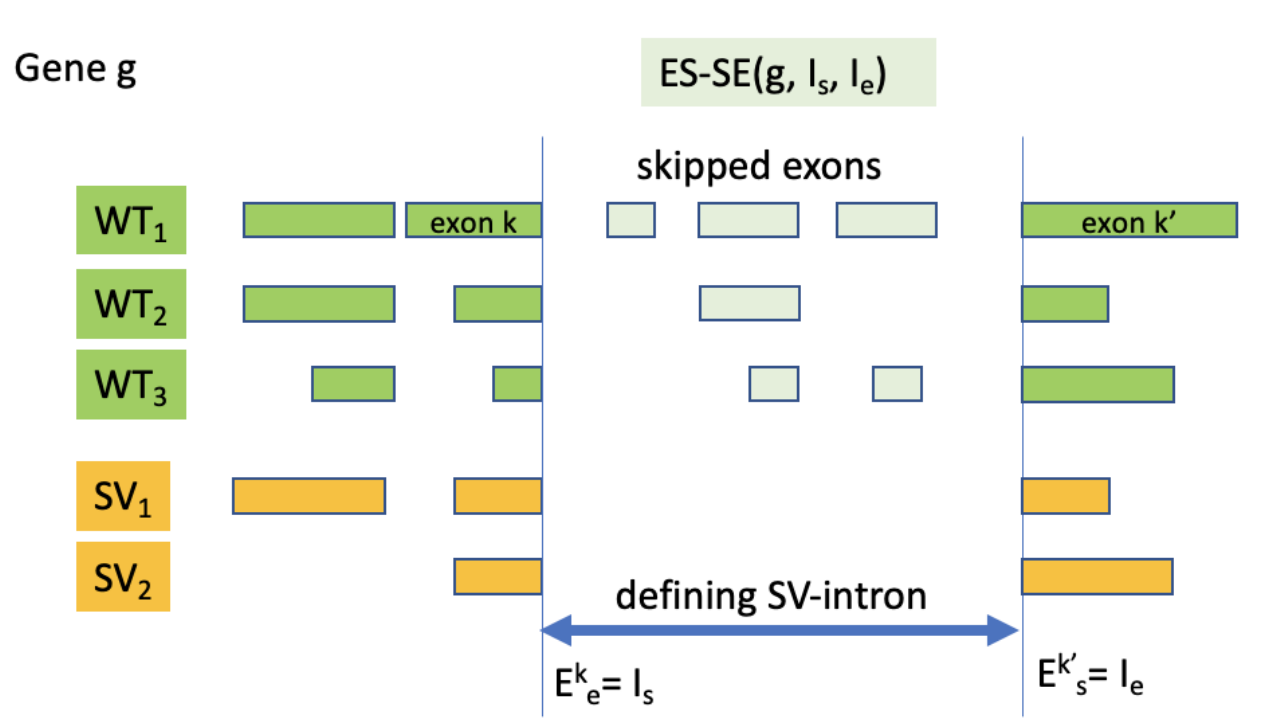
\includegraphics[width=1.0\textwidth]{figures/exonskipping/exon_skipping_diagram.png}
        \caption{Example of an Exon Skipping Event}
        \label{fig:exon_skip_diagram}
    \end{figure}

    The task is to identify exon-skipping events by processing Gene Transfer Format (GTF) files, which annotate the genome and provide information on the positions of genes, transcripts, exons, and coding sequences, among other structures. We will define an \textbf{Exon Skipping Event} (\(ES-SE\)) characterized by a gene g, an intron start \(I_s\), and an intron end \(I_e\). Each ES-SE requires at least two transcripts: a wildtype (WT) transcript and a splice variant (SV) of the same gene, which involves a specific intron. The defined intron spans from \(I_s\) to \(I_e\) and corresponds to a consistent exon end \(E_k^e\) and a consistent exon start \(E_{k'}^s\), where \(k'\) is greater than \(k\).

    The SVs associated with an ES-SE contain the specified intron\( [I_s, I_e)\), while the WTs may exhibit various combinations of skipped exons within the same intronic region. Importantly, all SVs lack non-skipped exons in the defined intronic region, distinguishing them from WTs.


    \section{Analysis}

    \subsection{1}
% to do, check for completion
% more on analysis file
%correctness, parsing correctness with analysis 20k protein coding, example was analyzed, correctness already explained, multiple people working on one problem

    \subsubsection{Structure}

    \paragraph{Program Usage}
    \begin{verbatim}
usage: java -jar ExonSkipRunner.jar [-h] -gtf <GTF file> -o <output file path>
                      [-a <analysis file path>]
named arguments:
  -h, --help             show this help message and exit
  -gtf <GTF file>        GTF file
  -o <output file path>  Output file
  -a <analysis file path>, --analysis <analysis file path>
                         (optional) File Path to the analysis file, gives
                         meta stats about exon skipping in this file
    \end{verbatim}

    \paragraph{Parsing}
    The general structure to store the information from a GTF file is as follows: A GTFAnnotation Object stores all the genes of a GTF in a Hash Map from GeneID to Gene Object. Each Gene has multiple transcripts, similarly stored in a HashMap from TranscriptID to Transcript Object. Additionally, all introns of a Gene are stored in a Tree Set (sorted by start position) on the gene level to avoid duplicate processing of Exon Skipping Events if there are multiple Splice Variants. Each Transcript has two TreeSets containing its respective Exons and Coding Sequences. For this assignment, we focused solely on the CDS entries; however, this structure was designed for maximum expandability and versatility, allowing for easy extension to accommodate other tasks in the future.

    The parsing of the GTF file is executed linearly, with each line processed sequentially. The parsing mechanism is robust and capable of handling files whose lines are not in the expected order; thus, a shuffled file can be processed just as effectively as a standard GTF file. The appropriate method handles the corresponding feature (gene, transcript, exon, or CDS) as each line is read. If an exon line is read before its associated gene has been processed (as seen in Homo\_sapiens.GRCh37.67, which lacks explicit gene or transcript entries), the gene\_id and transcript\_id attributes are utilized to create the necessary transcript and gene objects, which are then added to the GTF object. A similar approach is applied for transcripts and CDS entries when their parent objects have not yet been processed. A potential modification to the parsing process could involve calculating exon-skipping events immediately after a gene has been fully processed. This would reduce the need to retain multiple gene objects in memory. However, this approach relies on the assumption that the GTF file is always perfectly ordered, which could compromise the robustness of the parsing mechanism.

    \paragraph{Calculating Introns}
    Introns are calculated concurrently for each gene, with a new TreeSet initialized for each gene. The process involves iterating through the Coding Sequences of each transcript using a cursor, where a new intron is created for each interval between the end of the last CDS and the start of the next. This method ensures that all potential intron candidates, as defined in our Task, are accurately identified without duplication. Storing introns at the gene level (as opposed to the transcript level) effectively prevents redundancy, as the same intron may appear multiple times across different transcripts of a single gene.

    \paragraph{Analysis File} This program offers an additional option to generate an in-depth analysis file. The file is divided into two sections:
    \begin{enumerate}
        \item \textbf{General Metrics:} This section provides an overview of key statistics about the input file, such as the file length, the total time taken for processing, and specific times required for parsing, intron processing, exon processing, and output generation. Additionally, it includes cumulative counts of genes, transcripts, exons, and introns, as well as distinctions between genes/transcripts with and without coding sequences (CDS). The file also provides metrics on exon skipping events, gene lengths, and the average number of transcripts, exons, and CDS per gene.
        \item \textbf{Gene-Specific Details:} This section offers detailed information for each gene, including its identifier, name, length, the number of exon skipping events, and counts for transcripts, CDS, exons, and introns associated with the gene.
    \end{enumerate}
    The analysis files for all provided GTFs are located in:\\
    \texttt{/mnt/biocluster/praktikum/genprakt/kayser/Solution1/runs/*-anlysis.tsv}


    \begin{table}[H]
        \caption{Time Taken for each Dataset in ms}
        \label{tab:time-analysis}
        \resizebox{\textwidth}{!}{%
            \begin{tabular}{|l|l|l|l|l|l|l|}
                \hline
                \textbf{Dataset} &
                \textbf{File length} &
                \textbf{GTF Parsing} &
                \textbf{Intron processing} &
                \textbf{Exon processing} &
                \textbf{Output} &
                \textbf{Total} \\ \hline
                \textbf{gencode.v10.annotation}  & 2514768 & 8208  & 99 & 213 & 152 & 8678  \\ \hline
                \textbf{gencode.v25.annotation}  & 2579822 & 11266 & 63 & 200 & 170 & 11706 \\ \hline
                \textbf{Homo\_sapiens.GRCh38.90} & 2612848 & 10014 & 67 & 184 & 166 & 10436 \\ \hline
                \textbf{Mus\_musculus.GRCm38.75} & 1409515 & 4221  & 95 & 80  & 72  & 4474  \\ \hline
                \textbf{Homo\_sapiens.GRCh38.86} & 2575499 & 12645 & 60 & 202 & 178 & 13091 \\ \hline
                \textbf{Homo\_sapiens.GRCh38.93} & 2689571 & 10352 & 64 & 180 & 168 & 10770 \\ \hline
                \textbf{Homo\_sapiens.GRCh37.67} & 2246578 & 4657  & 79 & 273 & 197 & 5211  \\ \hline
                \textbf{Homo\_sapiens.GRCh37.75} & 2828317 & 7768  & 68 & 217 & 129 & 8188  \\ \hline
            \end{tabular}%
        }
    \end{table}


    Table \ref{tab:time-analysis} summarizes the time to process various GTFs in milliseconds, detailing the breakdown of time spent in different stages of the program's execution. Each GTF, including various annotations of the Homo sapiens and Mus musculus genomes, was processed multiple times to ensure consistent performance metrics.

    The results indicate that, although the execution times varied slightly across runs, the performance remained relatively consistent, highlighting the reliability of the implementation. The differences in the total processing time are often attributable to the size and complexity of the input files.

    For instance, the GTF \texttt{Homo\_sapiens.GRCh37.67} exhibits a notably shorter processing time. This may be due to its streamlined content, which only includes essential elements such as exons and coding sequences (CDS), thereby omitting the more complex gene lines. As a result, the program requires less computational effort when reading and processing this dataset, making it less intensive in this specific implementation.

    A significant observation from the table is that the GTF parsing step is the most time-consuming aspect of the entire process across all datasets by far. The time taken for intron and exon processing, while relevant, is significantly less than that for parsing, indicating that improvements in the parsing algorithm or methodology may yield the most substantial reductions in runtime.


    An analysis attempting to identify a clear pattern between runtime and specific aspects of the GTF file showed no definitive results. In Figure \ref{fig:length_vs_time_taken}, the file length (in lines) is plotted against the total processing time for outputting events. A slight correlation is observed, where longer files generally require more processing time. Other metrics, such as the number of CDS, introns, genes, exon-skipping events, introns per gene, and CDS per gene, were plotted against processing time, but none exhibited a clear and consistent correlation.
    \begin{figure}[H]
        \centering
        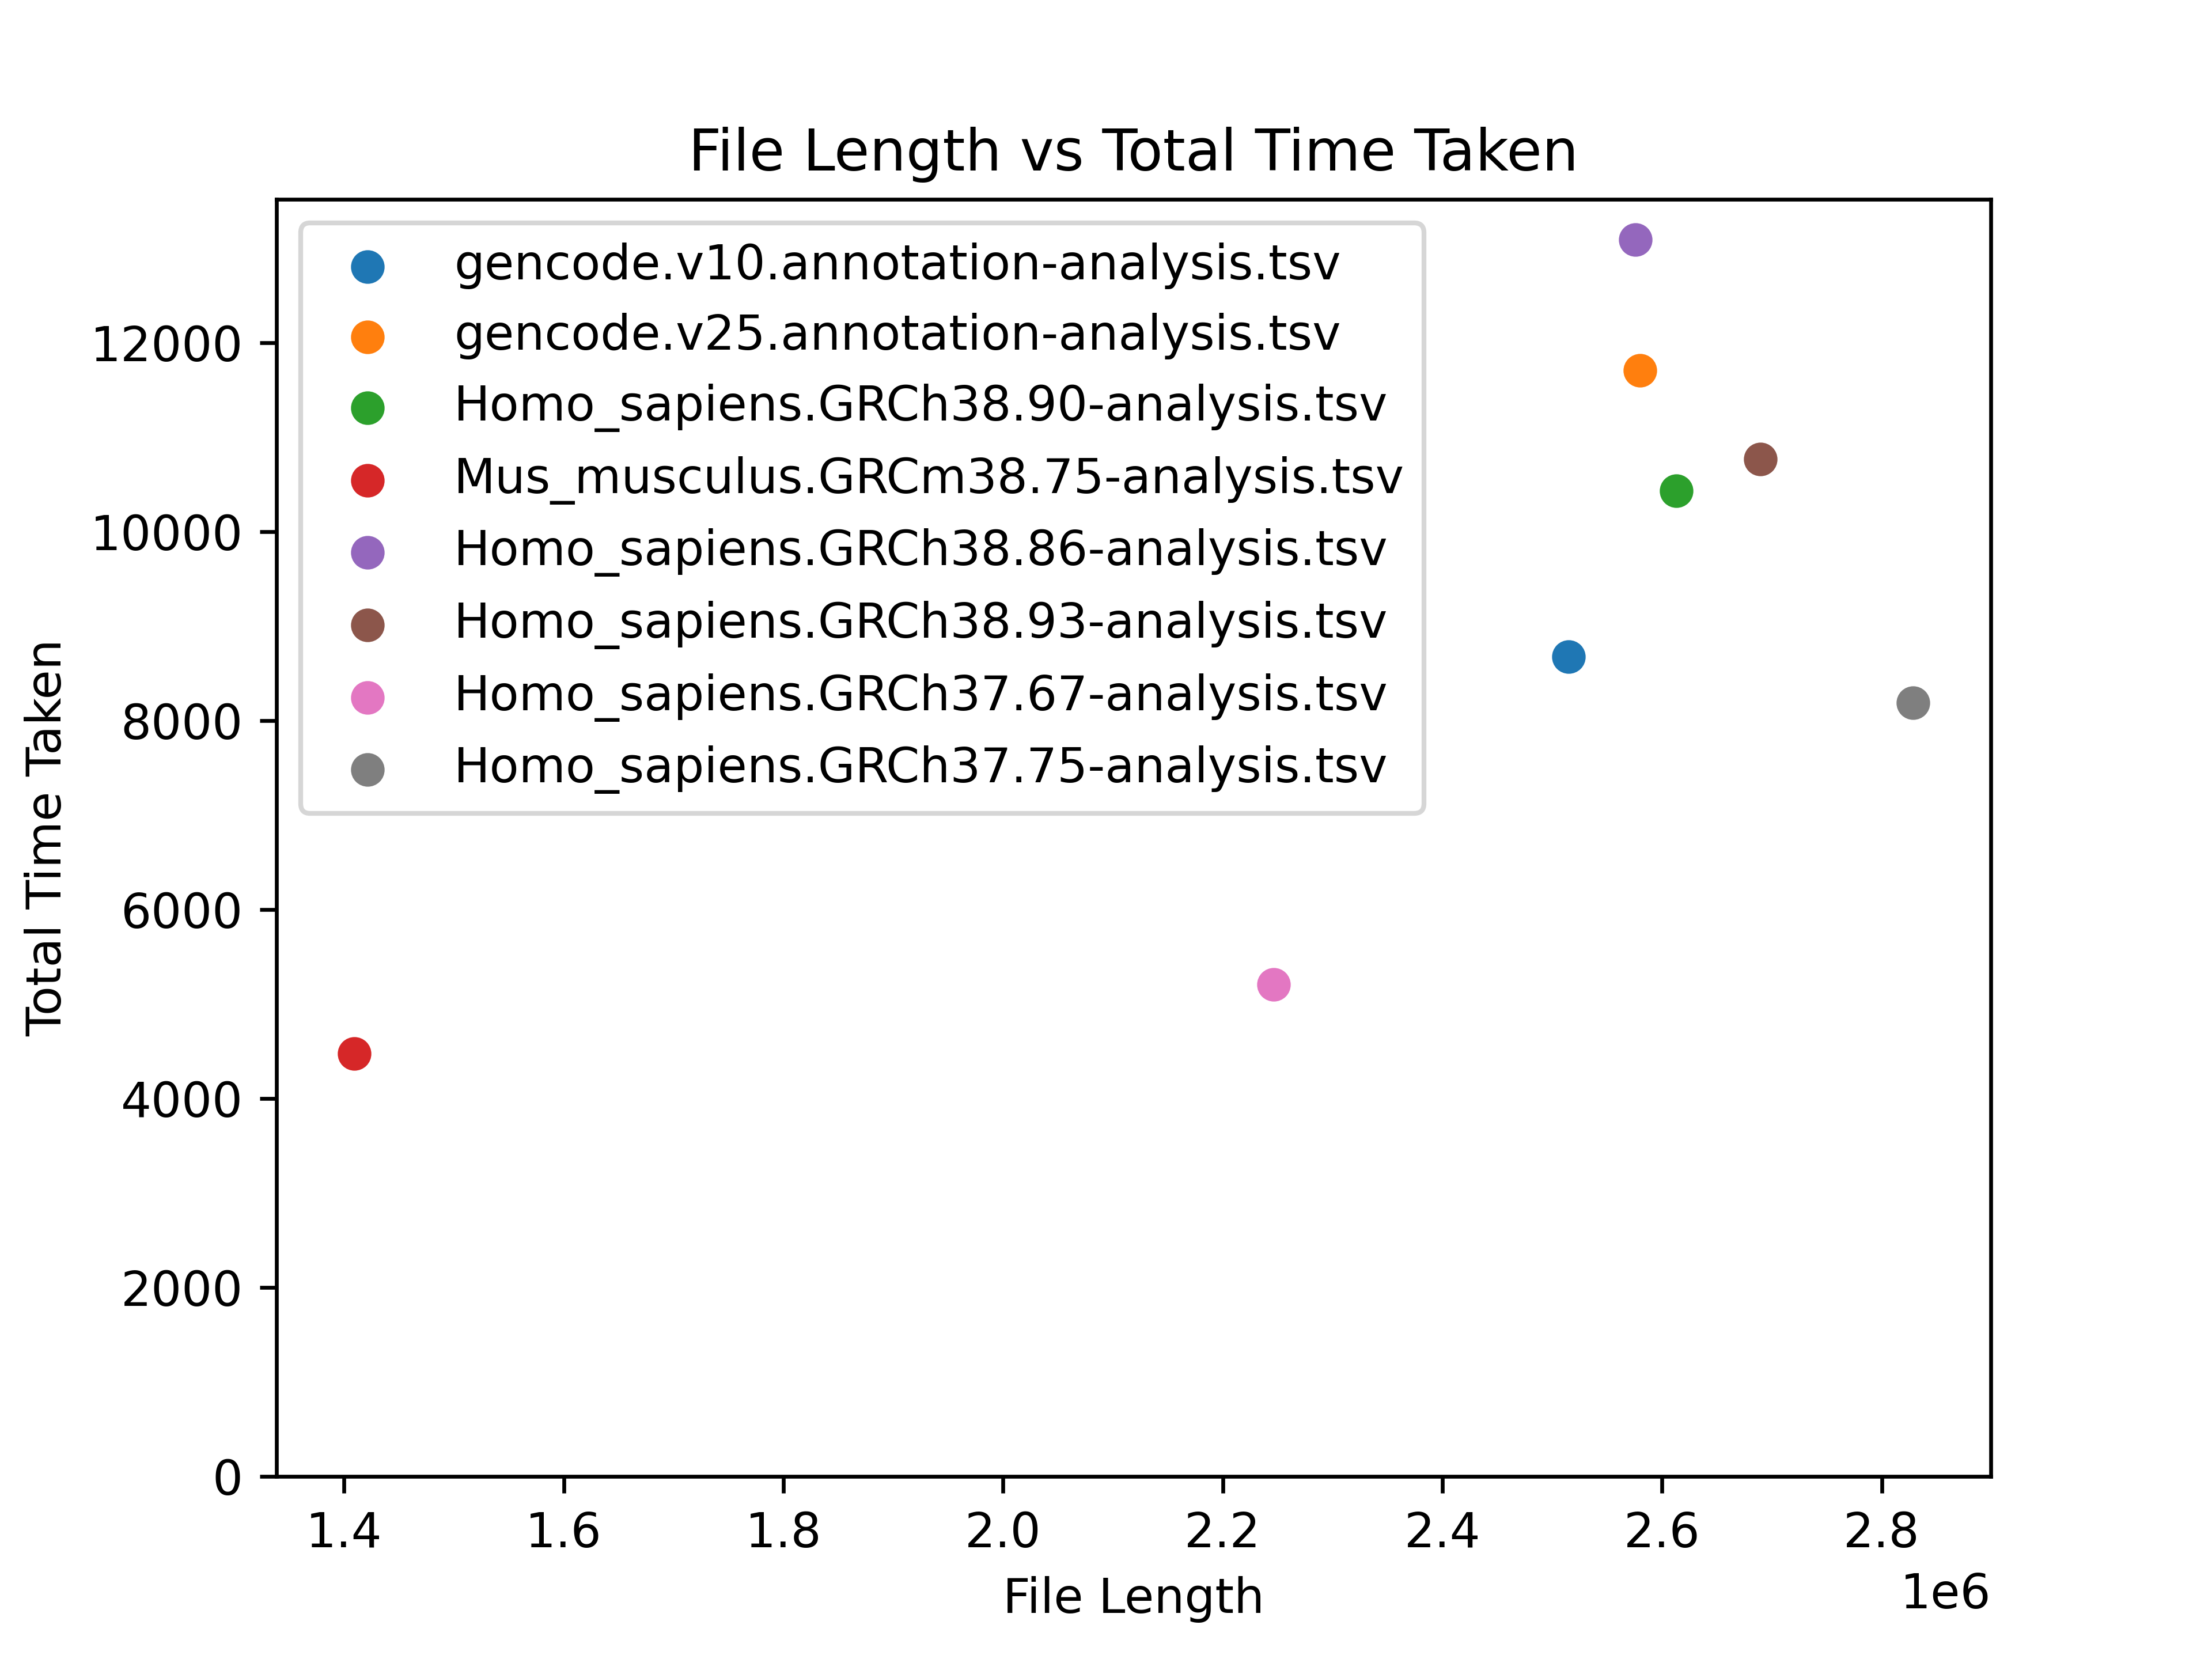
\includegraphics[width=0.5\textwidth]{figures/exonskipping/length_vs_time_taken}
        \caption{File Length vs Total Time Taken}
        \label{fig:length_vs_time_taken}
    \end{figure}

    \paragraph{Exon Skipping Splicing Events}
    In this approach, Exon Skipping Events are processed in parallel for each gene and stored in a list of ExonSkip events, which are outputted once all calculations are complete. While this approach is efficient for the files in this task, it could be modified to print each result as soon as it's ready to minimize memory usage.

    Each gene's intron candidate is evaluated to determine whether it qualifies as an Exon Skipping Event. This is achieved by iterating through all gene transcripts and checking each one for both SV and WT status. Each transcript’s coding sequences (CDS) are processed like intron checks (using a cursor iterator to access previous and current positions).

    During this process, two Boolean flags—\texttt{hasStartIntron} and \texttt{hasEndIntron}—are used to track whether the transcript contains an intron that starts and ends at the candidate intron’s positions. If these criteria are met, it’s considered an Exon Skipping Event. Additionally, any introns located inside the candidate intron are stored and added to the Wild Type (WT) set if the transcript is determined to be a WT. This is to ensure that any introns in the middle of an intron candidate but surrounded by two CDS are also found.

    The following steps outline the checks performed on each transcript’s introns to determine Exon Skipping Events:

    \begin{enumerate}
        \item \textbf{Exact Match with Candidate Intron}: If an intron is the same as the candidate intron, it qualifies as an SV, and processing can return immediately for this intron.
        \item \textbf{Start Intron Check}: If an intron starts at the candidate’s start position, \texttt{hasStartIntron} is set to \texttt{true}, and the intron is added to the \texttt{WTIntronsSet}.
        \item \textbf{End Intron Check}: If an intron ends at the candidate’s end position, \texttt{hasEndIntron} is set to \texttt{true}, and the intron is added to the \texttt{WTIntronsSet}.
        \item \textbf{Internal Intron}: If an intron lies entirely within the candidate intron, it is added to the \texttt{WTIntronsSet}.
    \end{enumerate}
    In the implementation, an optimization is applied before performing individual position checks on each intron. Instead of repeatedly checking each criterion, the program first verifies whether the intron lies within the start and end boundaries of the candidate intron (i.e., whether the start position of the intron is less than or equal to the start position of the candidate and the end position of the intron is greater than or equal to the candidate’s end position). Only if this initial boundary check passes are the start and end positions evaluated individually to confirm if both positions match, only one position matches, or neither matches. This optimization significantly reduces unnecessary comparisons, streamlining the detection process for Exon Skipping Events by narrowing down potential candidates early.

    Only if both \texttt{hasStartIntron} and \texttt{hasEndIntron} are \texttt{true} will the transcript be added to the WT set. This ensures that the correct WT introns are captured according to the set operations described. The \texttt{WTIntronsSet} is included in the main intron set only when a transcript is confirmed as WT, thereby excluding any erroneous introns from the main set. These four cases cover all possible scenarios, ensuring that all legitimate Exon Skipping Events are identified.

    After these steps, a final check confirms whether there is at least one SV and one WT, validating that the event is indeed an Exon Skipping Event and filtering out any false positives.

    To determine the minimum and maximum number of skipped bases and exons, each Wild Type transcript and its coding sequences are examined sequentially. Counters are initialized for each transcript to track the number of skipped exons and bases. If the current CDS is found within the candidate intron, the skipped exon counter increments by one, and the exon (CDS) length is added to the skipped bases counter. After iterating through all coding sequences of a transcript, the current minimum and maximum values for skipped exons and bases are updated as follows:

    \begin{minted}{java}
    currentMinSkippedExons = Math.min(currentMinSkippedExons, skippedExons);
    currentMaxSkippedExons = Math.max(currentMaxSkippedExons, skippedExons);
    currentMinSkippedBases = Math.min(currentMinSkippedBases, skippedBases);
    currentMaxSkippedBases = Math.max(currentMaxSkippedBases, skippedBases);
    \end{minted}

    This ensures that the minimum and maximum metrics are accurately calculated across all transcripts. Additional required attributes for each Exon Skipping Event, such as chromosome and strand information, are directly read from the gene. The \texttt{ntrans} value (number of transcripts) is accurately calculated because the program includes transcripts without coding sequences, which would not be possible if only CDS entries were read. The \texttt{nprots} value (number of transcripts with at least one coding sequence) is derived by counting the number of transcripts that contain at least one CDS.

    This approach ensures correctness through comprehensive checks at each step. By confirming both \texttt{hasStartIntron} and \texttt{hasEndIntron} conditions for a WT intron, only valid WT transcripts that span the candidate intron’s boundaries are considered. Internal introns are only included if they occur within the candidate, which aligns with typical exon-skipping definitions.

    The updating mechanism for minimum and maximum skipped exons and bases further ensures that the calculated values accurately represent all possible exon-skipping variations across transcripts. Including all transcripts, even those without CDS, provides a complete dataset for determining \texttt{ntrans} and \texttt{nprots}, preventing underestimating transcript counts. This robust approach reliably captures all Exon Skipping Events.

    Note: an interval tree could be used to optimize the calculations of the exon skipping events, but it is unnecessary to guarantee a quick runtime in this case. The parsing process takes around \~17 longer than the calculations of the exon skipping events, so for this task, it was not required but will be implemented in the future. The time taken for the major program sections as seen in Table \ref{tab:time-analysis} are always outputed, as well as potential errors

    \subsubsection{Correctness}
    In addition to the analysis performed during the calculation explanation, there are several further considerations for assessing the correctness of the program. While achieving 100\% on the submission server is a strong indication of correctness, it is not definitive proof. It is essential to consider the accuracy of the program on files not tested during development as well, ensuring robust calculations across varied data.

    For validation, one specific gene, \texttt{ENSG00000169715.14} (from \texttt{gencode.v25}), was selected and examined in detail for its events. The following analysis file excerpt provides context:
    \texttt{id=ENSG00000169715.14 name=MT1E length=1638 exon= skipping events=1 transcripts=3 cds=7 exons=7 introns=3}
    This gene has a single exon-skipping event, which includes one skipped exon with a total of 66 skipped bases. By thoroughly analyzing this event, the calculation of exon-skipping events was validated.

    However, performing a detailed examination on all 445,676 genes across the provided GTF files is impractical. Common pitfalls were also reviewed, such as avoiding duplicate entries for each exon-skipping event per structural variant (SV) and handling edge cases effectively.

    \subsection{2}

    \subsubsection{Structure}

    \paragraph{Program Usage}
    \begin{verbatim}
usage: Main [-h] -gtf <GTF file> -o <output file path>

Program that extracts all  ES-SE  defined  only  by  coding sequences (CDS)
listed in the input GTF file.

named arguments:
  -h, --help             show this help message and exit
  -gtf <GTF file>        GTF File Path
  -o <output file path>  Output Path
    \end{verbatim}

    \paragraph{Parsing}
    The parse method returns a "Genes" object, a wrapper for a map where the gene ID is the key and the gene object is the value. The wrapper is there for better readability; additional file metadata can be stored in this object if needed. A gene consists of the gene ID, optional properties (gene name, gene source, ...), and a map array. The array indices correspond to different features, while the gene ID is the key in the map. If necessary, an entry can be made for each distinct feature. A transcript stores its required and optional properties and contains a tree map with its feature records. The starting position is the key, and the feature records the value. Therefore, all feature records are sorted by starting position. The processing of each line runs parallel, but the genes structure is thread-safe, ensuring safe concurrent access and modification.

    Parsing is performed using a parallel stream, processing only lines with the feature types "CDS" and "exon". This approach significantly reduces the time and space needed, as lines without the desired features are neither processed nor stored in the genes structure. This is achieved by separating the lines until the feature column and checking if the feature type is valid. The split() method has been avoided to improve the performance further, and the separation of the different features and attributes is done manually. After that, the CDS and exon entries are inserted into the genes structure explained above. As gene ID and transcript ID are required attributes in a gtf file, the program first tries to get the gene out of the genes structure. If this is not possible, a new gene is initialized, its properties are set, and it is added to the genes map. It is possible to get 100\% on the submission server without reading the exons. This also improves the runtime by a few seconds. However, to get the right amount of transcripts (nTrans), the exons must also be read in.

    \paragraph{Calculating Introns}
    Introns are calculated for each gene by going through every transcript of the gene. As each transcript has its coding sequences stored and sorted by starting position in a treemap, it is possible to go through the map entries and calculate the gaps between each coding sequence to retrieve the introns. After all the introns are calculated, they are stored in two different data structures - an interval tree and a set with unique introns. The uniqueness of an intron is defined by its start and stop position. The introns are calculated asynchronously. A future is created and added to a list for every transcript in the gene. After that, introns are saved in the two structures by iterating over the futures and getting the introns. This way, maximizing parallel and asynchronous computations is possible, as the main thread does not have to wait for every intron list before going to the subsequent transcript. Before going to the ES-SE computations, the size of the CDS and exon map is stored and passed to the "calculateEsSe" method to get the correct values for the "nTrans" and "nProts" properties.

    \paragraph{Exon Skipping Splicing Events}
    After the introns for a gene are calculated, the two retrieved data structures - the interval tree with all introns for the gene and the set with the unique introns for the gene - are used to calculate all ES-SE for the current gene. Every unique intron is a candidate for being a splicing variant. As all introns for the genes are stored in an interval tree, it is possible to check which introns are spanned by the candidate intron. The result is stored in a map where the introns are stored by transcript. This map is a new data type called "IntronByTranscriptMap" that implements the collection interface. It is implemented because the library used for the interval tree needs a collection to store the introns found in it. Maps are typically not suitable. When adding an intron to the new data type it is added with its transcript ID as the key to the private hash map in the background. The interval tree is a good fit for this use case, as it provides the introns that are needed very efficiently wrapped in one method call. With the following two lines all the introns that the candidate spans can be retrieved:
    \begin{minted}{java}
var intronsSpannedByCandidate = new IntronByTranscriptMap();
intronsForGene.getIntervalsSpannedBy(candidateIntron.getStart(),
    candidateIntron.getStop(), intronsSpannedByCandidate);
    \end{minted}
    What is left to check for each transcript is whether it contains a splicing variant (SV) or a wild type (WT). If there is more than one intron per transcript, this indicates a potential wild type for the transcript. Now, this transcript's introns are compared to the candidate intron. If there is an intron with the same start position and a different intron with the same stop position as the candidate intron, it is accepted as a wild type. If there is only one intron in the list returned by the introns by transcript map, and this intron has the same start and stop position as the candidate intron, it is accepted as a splicing variant. Transcripts that contain neither a SV nor a WT are removed from the list so that the statistic that will be calculated later is accurate.

    \begin{table}[H]
        \caption{Time Taken for each Dataset in ms}
        \label{tab:2-time-analysis}
        \resizebox{\textwidth}{!}{%
            \begin{tabular}{|l|l|l|l|l|l|l|}
                \hline
                \textbf{Dataset} &
                \textbf{File length} &
                \textbf{GTF Parsing} &
                \textbf{Intron \& ES-SE processing} &
                \textbf{Output} &
                \textbf{Total} \\ \hline
                \textbf{gencode.v10.annotation}  & 2514768 & 8560  & 529 & 91  & 9180  \\ \hline
                \textbf{gencode.v25.annotation}  & 2579822 & 11444 & 533 & 136 & 12113 \\ \hline
                \textbf{Homo\_sapiens.GRCh38.90} & 2612848 & 10275 & 537 & 126 & 10938 \\ \hline
                \textbf{Mus\_musculus.GRCm38.75} & 1409515 & 4523  & 406 & 78  & 5007  \\ \hline
                \textbf{Homo\_sapiens.GRCh38.86} & 2575499 & 12862 & 496 & 119 & 13477 \\ \hline
                \textbf{Homo\_sapiens.GRCh38.93} & 2689571 & 10750 & 557 & 109 & 11416 \\ \hline
                \textbf{Homo\_sapiens.GRCh37.67} & 2246578 & 5146  & 559 & 112 & 5817  \\ \hline
                \textbf{Homo\_sapiens.GRCh37.75} & 2828317 & 7863  & 550 & 123 & 8536  \\ \hline
            \end{tabular}%
        }
        Table \ref{tab:2-time-analysis} summarizes the time to process various GTFs in milliseconds, detailing the breakdown of time spent in different stages of the program's execution. Each file was processed multiple times to maintain consistent metrics.
        The time required for calculating the ES-SEs and saving them to a file remained constant, regardless of the file size. The parsing time of the Homo\_sapiens.GRCh38.86 file dropped from 12,993 ms to 3,112 ms after caching. The times shown in the table reflect pre-caching performance, as the file would likely not be cached in a real-world scenario. Even when the files are already cached, parsing remains the most time-consuming part of the entire program. This suggests that further optimizations in the parsing process offer the greatest potential for reducing overall processing time.
    \end{table}

    The bases skipped for each ES-SE are calculated by taking the splicing variant's length and subtracting the length of all the introns in the transcript. For calculating the skipped exons, it is possible to take the size of the read-in transcript ID to introns map. This is the only reason the exons have to be saved as well. The WT proteins are derived after all transcripts have been checked, and now every entry in the intron by transcript map is either a SV or a WT. By iterating over the values of this map and checking if the transcript contains more than one intron, we can check if it is a WT. If the intron list only contains one item, it is another SV and will be added to the SV-Proteins list. In some edge cases, the protein ID is not given. In this case, the program will leave the SV prots and WT prots column empty. After the statistics are calculated, the ES-SE is added to a list containing all ES-SE for the current gene. It is first added to a local list to minimize the time the global list is locked. This way, the method can run efficiently asynchronously for every gene. This whole method runs parallel and asynchronous because the ES-SE collection is also thread-safe.

    \paragraph{Logging} Logging is implemented and informs about success, eventual warnings, and errors, as well as the time that was spent parsing, calculating introns, exon skipping, and writing to a file. It is especially useful since the log file can also be accessed in the results on the submission server. Additionally, the logs can be seen in the console.

    \subsubsection{Correctness}

    \paragraph{Definition of the Problem}
    A splicing variant has an intron with specific start and stop positions. In the same gene, there must be at least one other transcript that contains at least two exons inside of the region of the candidate SV. Such transcripts are called wild types if there is one exon with the same start position as the intron of the splicing variant and another exon with the same stop position. There can be additional exons in between, but this is not required.

    \textbf{IMPORTANT}: A splicing variant is only referred to as such if there are corresponding wild types.

    \paragraph{ES-SE Calculation}
    The program is correct because:

    The process iterates through each gene and considers only the transcripts of the respective gene for the calculation. It uses all unique introns to search for potential splicing variants. An intron is considered identical to another if they have the same start and stop positions. This definition is used because a splicing variant (SV) has specific start and end positions.

    Each of these candidate introns are then examined by only using coding sequences that are within the start and stop range of the candidate intron using an interval tree and store them by transcript id in a map.

    Then, checking if each transcript entry qualifies as a WT is necessary. Two flags are used for this: hasStart and hasStop. If both are true, meaning there are two different CDSs in the same transcript that match the start and stop positions of the candidate intron, the candidate is an ES-SE. There can be other exons between these two, though this is only sometimes the case.

    If a transcript returned by the interval tree does not contain a wild type, it is removed from the map. There may also be multiple transcripts possessing the SV. This scenario is handled by checking the number of CDSs in the respective transcripts the interval tree returns. If there is only one entry, it can be a splicing variant or an entry that needs to be removed. If this CDS has the same start and stop positions as the candidate intron, it is not removed from the list and is later included in the SV proteins.

    After these steps, the map of the introns that are spanned by the candidate introns are either SVs or WTs. Thus, the calculation of whether a candidate intron is an SV is accurate.

    \paragraph{Statistics for the Output}
    Now, it is necessary to loop through the obtained map of SVs and WTs, where the transcript ID is the key.
    The only thing that is not trivial in this section is how the skipped bases and exons are calculated. The skipped bases are calculated by taking the total length of all introns present in the respective transcript and subtracting it from the size of the SV. This gives the length of all CDS not included in the SV, representing the number of skipped bases.
    The number of skipped exons is determined by taking the size of the intron list for each transcript and subtracting one. If there is only one intron, there are no skipped exons, as the intron itself represents an SV. If there are two introns, it indicates a gap between them, where an exon is located. Each additional intron introduces another gap, corresponding to an additional skipped exon. So, for each additional intron, the number of skipped exons increases by one.

    \subsubsection{Time Complexity}
    All the code shown in this section is very simplified.

    \paragraph{Parsing}
    The parsing is done linearly, with each line being read in parallel. However, this does not affect the time complexity. The processing of each line consists of three for-loops and map operations. The map operations get, put, and computeIfAbsent all have a time complexity of $O(1)$. The three for-loops are executed sequentially and look as follows:

    \begin{lstlisting}[language=Java]

1. for (int i = 0; i < line.length(); i++) { ... }
2. for (int i = 0; i < splitLine[8].length(); i++) { ... }
3. for (var attribute : attributes) { 
    for (int i = 0; i < attribute.length(); i++) { ... } 
}

    \end{lstlisting}
    The first loop reads each character of the line sequentially and stores the content in the corresponding fields of the splitLine array. The second loop splits the attributes and stores them in an attribute list. The third loop iterates over the attributes and stores them in the corresponding gene, transcript, or feature records.

    The first loop has a time complexity of $O(n)$, where n is the line length. Parsing the attributes also has a complexity of $O(n)$ because the total length of the attributes is at most n. The third loop again processes all characters in the attributes, resulting in an overall complexity of $O(3n)$, simplifying to $O(n)$.

    \paragraph{ES-SE Computation}
    The outer for loop iterates over all genes (G). Inside of this loop are two computations:

    \begin{enumerate}
        \item Intron Calculation
        \item ES-SE Calculation
    \end{enumerate}

    \textbf{Intron Calculation} To compute the introns, it is necessary to go over every transcript (T) in the gene and then iterate over every CDS (C) in the transcript, which makes a time complexity of $O(T * C) $ and an overall complexity of $O(G * T * C)$. Significantly simplified, it looks like this:

    \begin{lstlisting}[language=Java]
for (var geneEntry : data.getFeaturesByTranscriptByGene()) {
    for (var transcriptEntry : transcriptCdsMap) {
        for (var cds : cdsMap.getTranscriptEntry().getPositions()) { ... }
    }
}
    \end{lstlisting}

    \textbf{ES-SE Calculation} For simplicity, the maximum unique introns are considered the maximum number of computed introns (I).

    The unique introns (I) are iterated over in the first for loop. Then, the introns spanned by the unique intron are retrieved using the interval tree. Since it is unclear how the interval tree is implemented, a query time of $O(log I)$ is assumed based on a standard implementation. This list is then iterated over again to check for SV or WT, resulting in a runtime of $O({I}^2)$. The query time of the interval tree can be ignored as this process would only have a time complexity of $O(I * log I)$.

    \begin{lstlisting}[language=Java]
for (var candidateIntron : setWithUniqueStartAndStopIntrons) {
    for (var spannedByEntry : copyOfSpannedByEntrySet) 
        { ... }
}
    \end{lstlisting}

    The last two loops are nested and iterate over a reduced or equally sized list of introns retrieved from the interval tree. They calculate the skipped exons, bases, and WT \& SV proteins. The two loops review all the introns spanned by the candidate intron. IntronsSpannedByCandidate is of a custom data type that stores the introns with the transcript ID as the key in a map. This is why the nested loop is necessary. In conclusion, the complexity here is also $O(I^2)$ as all the candidate introns go over all the introns from the spanned-by-candidate list. This means the complexity of the computation of the ES-SEs after the introns are calculated is $O(I^2)$, which equals $O((T * C)^2)$.

    \begin{lstlisting}[language=Java]
for (var intronWithSV : intronsSpannedByCandidate) {
    for (var currentIntron : intronList) { ... }
}
    \end{lstlisting}

    Therefore, the overall complexity of the method is $O(G * ((T*C) + (T*C)^2))$.

    \subsection{Top Genes}

    While searching for the top 10 genes with the highest number of base and exon skips, we noticed that gene IDs sometimes include versions in the format Gene-ID.XX. These versions were omitted here.

    What can be seen in Tables \ref{tab:bases-skipped} and \ref{tab:exons-skipped} is that the top two genes code for the protein titin in both \href{https://www.uniprot.org/uniprotkb/Q8WZ42/entry}{humans} and \href{https://www.uniprot.org/uniprotkb/A2ASS6/entry}{mice}.

    \begin{table}[H]
        \caption{Top 10 Genes by Maximum Bases Skipped}
        \label{tab:bases-skipped}
        \begin{center}
            \begin{tabular}{ |p{2cm}|p{4cm}|p{2cm}| p{2.5cm}|  }
                \hline
                Symbol  & Gene-ID                                                                                           & Bases & Species      \\
                \hline
                TTN     & \href{https://www.ensembl.org/Homo_sapiens/Gene/Summary?g=ENSG00000155657}{ENSG00000155657} & 26106 & Homo Sapiens \\
                Ttn     & \href{https://www.ensembl.org/mus_musculus/Gene/Summary?g=ENSMUSG00000051747}{ENSMUSG00000051747}   & 24843 & Mus Musculus \\
                TTN     & \href{https://www.ensembl.org/Homo_sapiens/Gene/Idhistory?g=ENSG00000283186}{ENSG00000283186} & 22134 & Homo Sapiens \\
                MUC4    & \href{https://www.ensembl.org/Homo_sapiens/Gene/Summary?g=ENSG00000145113}{ENSG00000145113} & 12875 & Homo Sapiens \\
                ADGRV1  & \href{https://www.ensembl.org/Homo_sapiens/Gene/Summary?g=ENSG00000164199}{ENSG00000164199} & 12530 & Homo Sapiens \\
                DYNC2H1 & \href{https://www.ensembl.org/Homo_sapiens/Gene/Summary?g=ENSG00000187240}{ENSG00000187240} & 10182 & Homo Sapiens   \\
                Fsip2   & \href{https://www.ensembl.org/mus_musculus/Gene/Summary?g=ENSMUSG00000075249}{ENSMUSG00000075249} & 9659 & Mus Musculus \\
                NBPF20  & \href{https://www.ensembl.org/Homo_sapiens/Gene/Idhistory?g=ENSG00000203832}{ENSG00000203832} & 9573 & Homo Sapiens \\
                FSIP2   & \href{https://www.ensembl.org/Homo_sapiens/Gene/Summary?g=ENSG00000188738}{ENSG00000188738} & 9437 & Homo Sapiens \\
                XIRP2   & \href{https://www.ensembl.org/Homo_sapiens/Gene/Summary?g=ENSG00000163092}{ENSG00000163092} & 9379 & Homo Sapiens \\
                \hline
            \end{tabular}
        \end{center}
    \end{table}

    \begin{table}[H]
        \caption{Top 10 Genes by Maximum Exons Skipped}
        \label{tab:exons-skipped}
        \begin{center}
            \begin{tabular}{ |p{2cm}|p{4cm}|p{2cm}| p{2.5cm}|  }
                \hline
                Symbol  & Gene-ID                                                                                           & Exons & Species      \\
                \hline
                TTN     & \href{https://www.ensembl.org/Homo_sapiens/Gene/Summary?g=ENSG00000155657}{ENSG00000155657} & 169 & Homo Sapiens \\
                Ttn     & \href{https://www.ensembl.org/mus_musculus/Gene/Summary?g=ENSMUSG00000051747}{ENSMUSG00000051747}   & 154 & Mus Musculus \\
                TTN     & \href{https://www.ensembl.org/Homo_sapiens/Gene/Idhistory?g=ENSG00000283186}{ENSG00000283186} & 121 & Homo Sapiens \\
                NBPF20  & \href{https://www.ensembl.org/Homo_sapiens/Gene/Idhistory?g=ENSG00000203832}{ENSG00000203832} & 78 & Homo Sapiens \\
                DYNC2H1 & \href{https://www.ensembl.org/Homo_sapiens/Gene/Summary?g=ENSG00000187240}{ENSG00000187240} & 70 & Homo Sapiens \\
                NBPF10  & \href{https://www.ensembl.org/Homo_sapiens/Gene/Summary?g=ENSG00000271425}{ENSG00000271425} & 70 & Homo Sapiens   \\
                NBPF10  & \href{https://www.ensembl.org/Homo_sapiens/Gene/Idhistory?g=ENSG00000163386}{ENSG00000163386} & 60 & Homo Sapiens \\
                ADGRV1  & \href{https://www.ensembl.org/Homo_sapiens/Gene/Summary?g=ENSG00000164199}{ENSG00000164199} & 59 & Homo Sapiens \\
                NBPF20  & \href{https://www.ensembl.org/Homo_sapiens/Gene/Summary?g=ENSG00000162825}{ENSG00000162825} & 56 & Homo Sapiens \\
                NBPF12  & \href{https://www.ensembl.org/Homo_sapiens/Gene/Idhistory?g=ENSG00000186275}{ENSG00000186275} & 52 & Homo Sapiens \\
                \hline
            \end{tabular}
        \end{center}
    \end{table}

    \subsection{Skipping Analysis}

% required plots
    In Figure \ref{fig:cum-max-skipped-bases}, the cumulative distribution of the maximum skipped bases per exon skipping event by file is shown.
% Patterns the same across all datasets
% Steep initial rise indicates most exon-skipping events involve a small number of skipped bases (typically under 100).
% Curves flatten as the number of skipped bases increases, suggesting larger exon-skipping events are rare.



    \begin{figure}
        \centering
        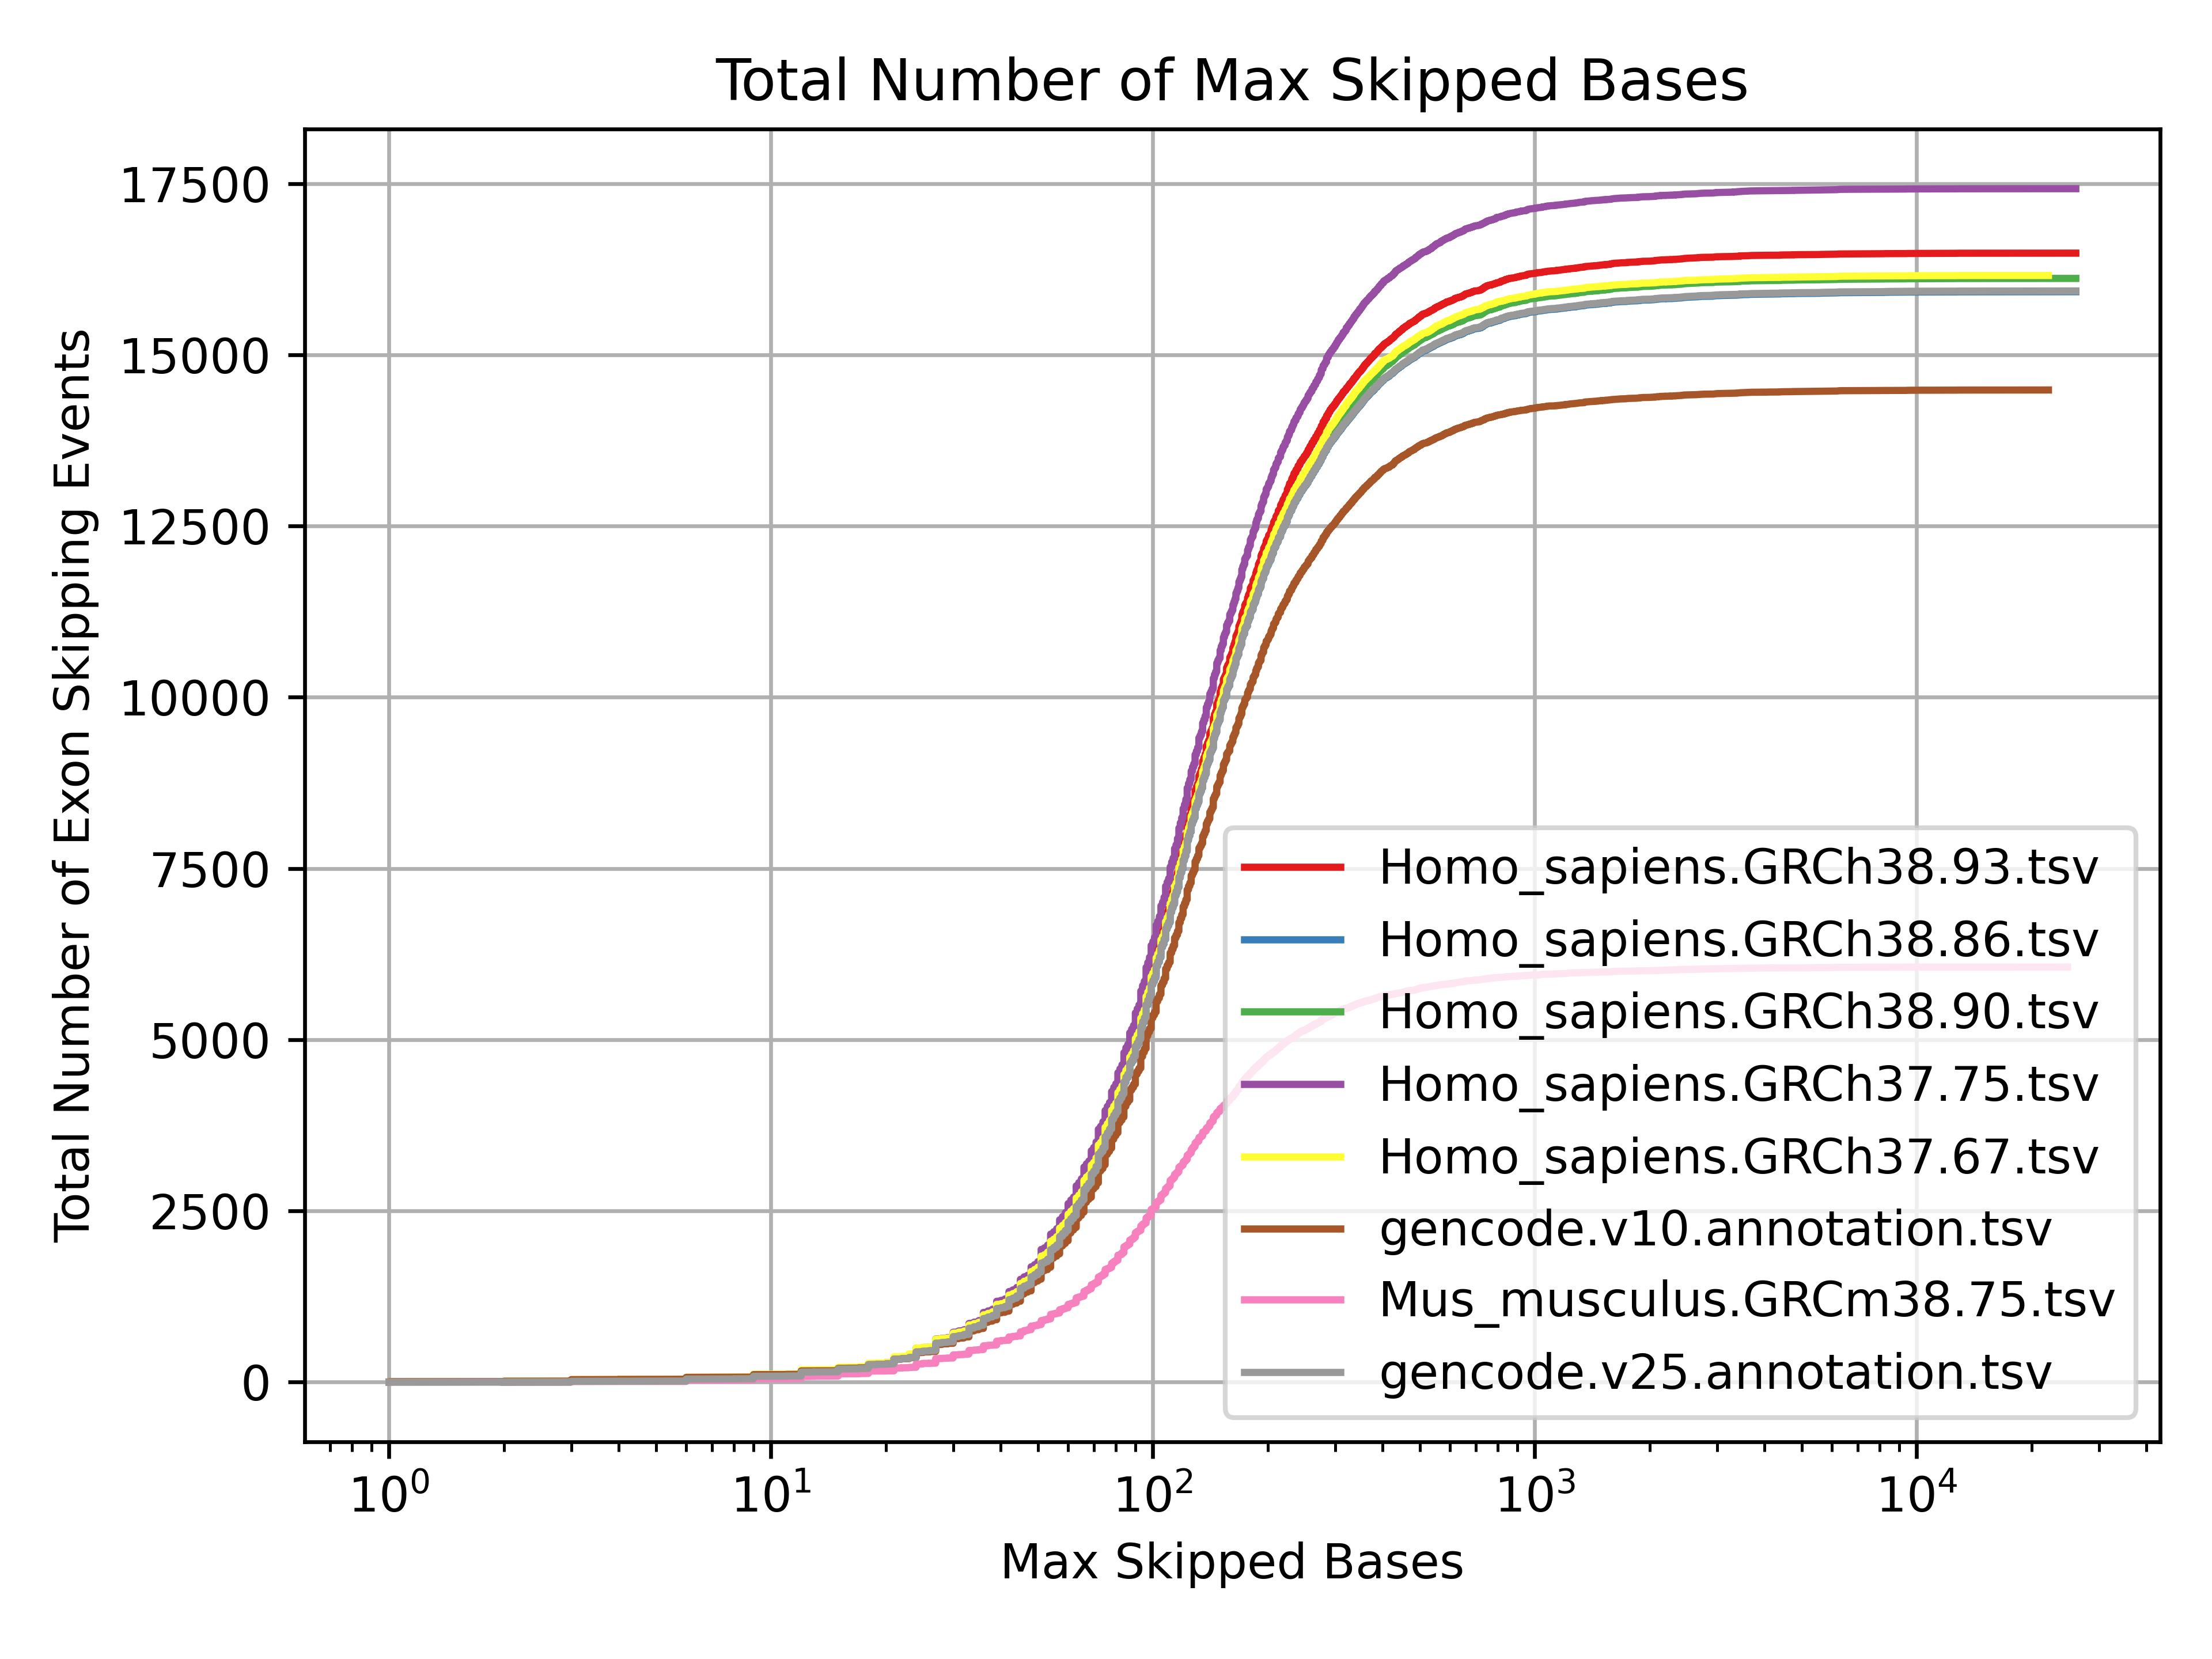
\includegraphics[width=0.7\textwidth]{figures/exonskipping/skipped_bases.jpg}
        \caption{Cumulative Plot of maximum skipped bases}
        \label{fig:cum-max-skipped-bases}
    \end{figure}


    In Figure \ref{fig:cum-max-skipped-exons}, the cumulative distribution of the maximum skipped exons per exon skipping event by file is plotted.
% Patterns the same across all datasets
% Sharp increase at lower skipped exon counts shows most events involve fewer than 10 exons.
%Curves plateau beyond this point, highlighting the rarity of events with many skipped exons.

    \begin{figure}
        \centering
        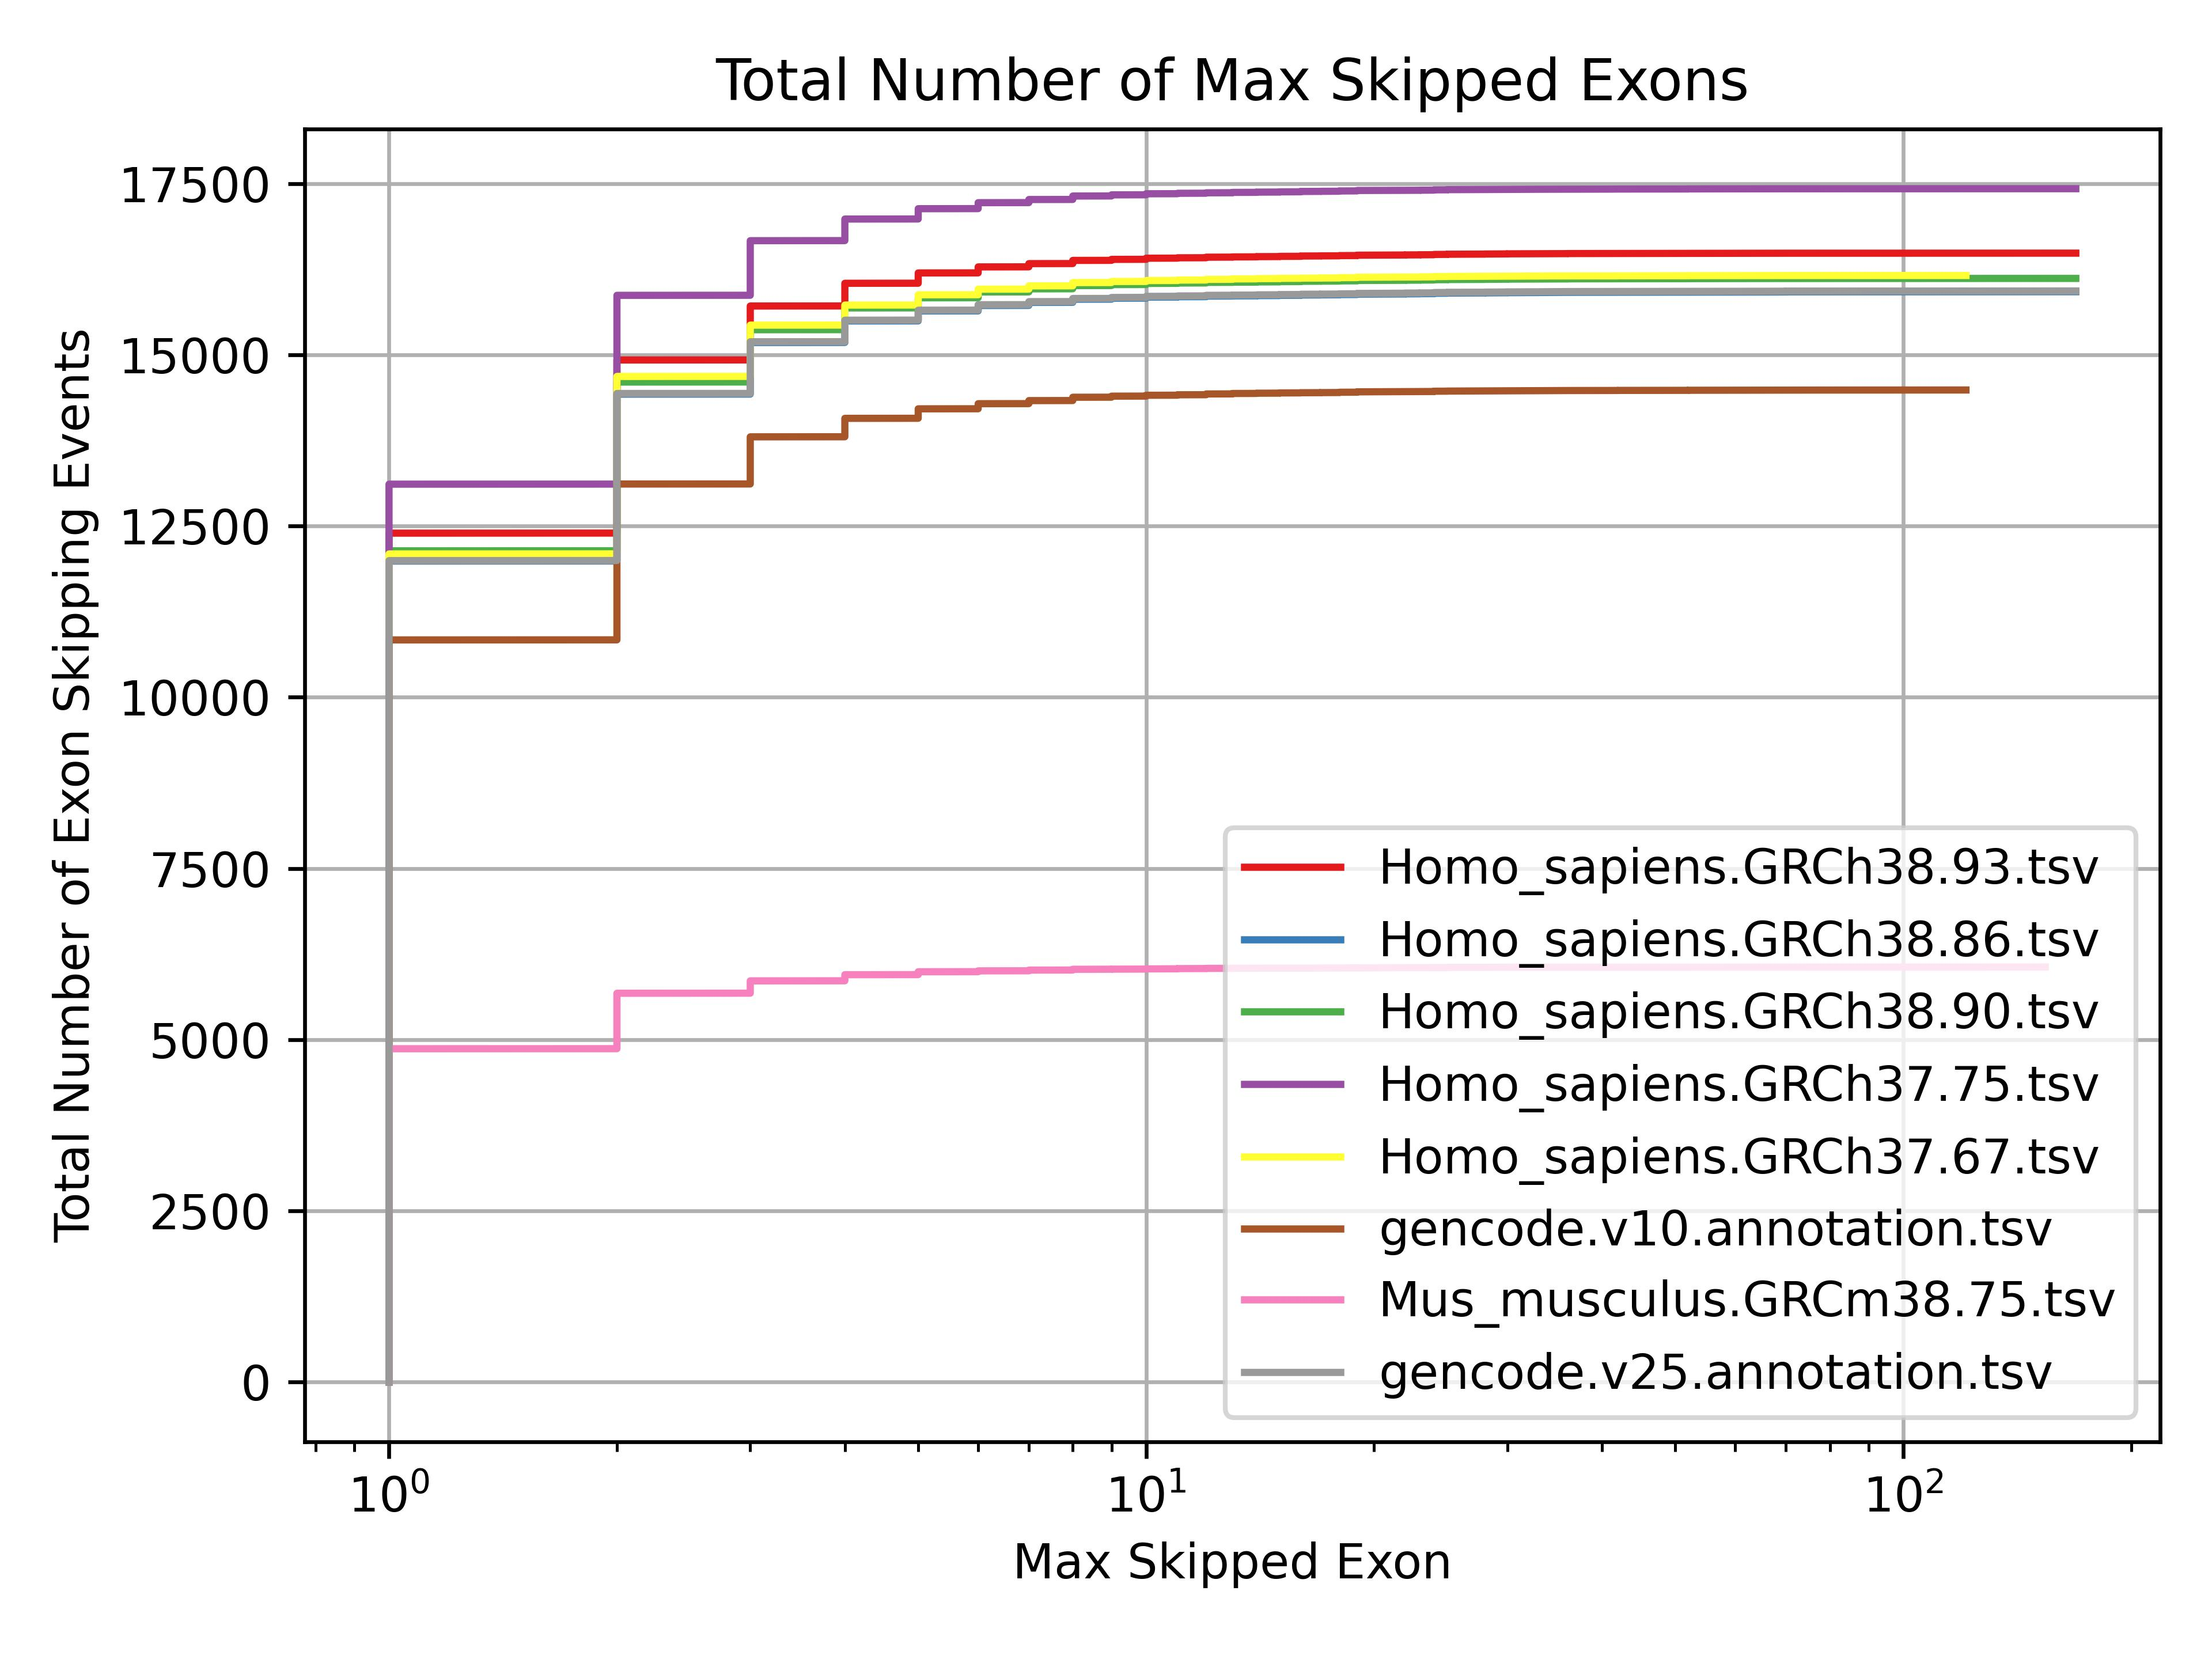
\includegraphics[width=0.7\textwidth]{figures/exonskipping/skipped_exons.jpg}
        \caption{Cumulative Plot of maximum skipped exons}
        \label{fig:cum-max-skipped-exons}
    \end{figure}


    In Figure \ref{fig:cum-exon-skips}, the cumulative distribution of exon-skipping events across the protein-coding genes is shown. From the plot, it is evident that the majority of protein-coding genes across datasets exhibit no exon-skipping events, as indicated by the sharp initial rise in each curve. For genes that do exhibit exon-skipping, most have only a few events, typically within the range of 1 to 5. Beyond 5 events, the curves level off significantly, indicating that exon-skipping is relatively rare in higher counts. This pattern is consistent across all datasets, with only slight variations in the exact counts of genes with exon-skipping events. This suggests that exon-skipping is an infrequent phenomenon within individual genes, and most protein-coding genes are minimally affected by such events. Overall, the figure highlights the sparsity of exon-skipping events, emphasizing that while they do occur, they are generally limited to a small subset of genes and events per gene.



    \begin{figure}
        \centering
        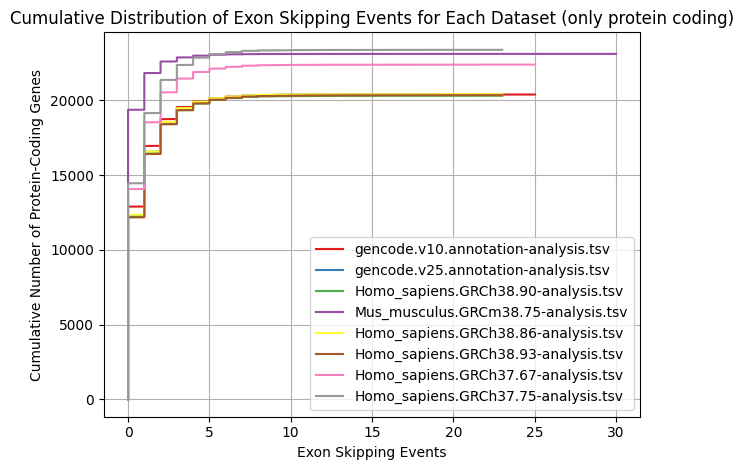
\includegraphics[width=0.7\textwidth]{figures/exonskipping/cumulative_exon_skipping_events}
        \caption{Cumulative Plot of Exon Skipping Events}
        \label{fig:cum-exon-skips}
    \end{figure}


% Correctness analyis?
% Plot ideas: skips per gene?
% Analyze one specific example 
% Multiple different people working on one problem independtly??


% edge cases
% no protein-id in gencode-v10
% When the entries aren't in the correct order (- strand)
\end{document}
